\documentclass{beamer}

\usepackage{amsmath}
\usepackage{float}
\usepackage{graphicx}
\usepackage{color}
\usepackage{url}
\usepackage{ulem}
\usepackage{ctex}

\newcommand{\red}[1]{\textcolor{red}{#1}}
\newcommand{\blue}[1]{\textcolor{blue}{#1}}

\usetheme{CambridgeUS}

\title{CS100 Recitation 1}
\author{Dinghao Cheng}
\institute{ \textbf{Special thanks: GKxx}}
\date{Februrary 22, 2022}

\begin{document}

\begin{frame}
    \titlepage
\end{frame}

\AtBeginSubsection[]{
    \begin{frame}{Contents}
        \tableofcontents[currentsection, currentsubsection]
    \end{frame}
}

\section{Before class}
\begin{frame}{Useful website}
    \begin{itemize}
        \item \url{https://i-techx.github.io/dashboard}
        \item Courses information in ShanghaiTech
        \item The website is hosted on Github Pages, so sometimes you may need VPN...
    \end{itemize}
\end{frame}
\section{Foundations of C - have a glance}

\subsection{Language Standards}

\begin{frame}{Language Standards}
    \begin{itemize}
        \item Standards of C: C89/90, C99, C11, C17, C23 (coming soon).
        \item Standards of C++: C++98/03, C++11, C++14, C++17, C++20, C++23 (coming soon),\dots
        \pause
        \item A new version of standard C++ comes out every \blue{three} years.
        \pause
        \item To specify a standard for the compiler, use \texttt{-std=c}\(x\) or \texttt{-std=c++}\(y\), e.g. \texttt{-std=c11}, \texttt{-std=c++17}.
        \pause
        \item To see what language standard the compiler is using, check the macro \texttt{\_\_STDC\_VERSION\_\_} in C and \texttt{\_\_cplusplus} in C++. For example, \texttt{\_\_cplusplus == 201703L} means that the program is compiled under C++17.
    \end{itemize}
\end{frame}

\subsection{Arithmetic Types}

\begin{frame}{Integer Types}
    \begin{itemize}
        \item \texttt{short (int), signed short (int), unsigned short (int)}
        \item \texttt{int, signed int, unsigned int}
        \item \texttt{long (int), signed long (int), unsigned long (int)}
        \item \texttt{long long (int), signed long long (int), unsigned long long (int)} (since C99)
    \end{itemize}
\end{frame}

\begin{frame}{Integer Types}
    \begin{itemize}
        \item What's the size of a \texttt{short}? \texttt{int}? \texttt{long}? \texttt{long long}?\\
        \pause
        \blue{\texttt{short} and \texttt{int} are at least 16-bit. \texttt{long} is at least 32-bit. \texttt{long long} is at least 64-bit.}\\
        \blue{\texttt{1 == sizeof(char) <= sizeof(short) <= sizeof(int) <= sizeof(long) <= sizeof(long long)}}
        \pause
        \item Do \texttt{int} and \texttt{signed int} name the same type? What about others?
        \pause
        \blue{For any integer type \texttt{T}, \texttt{T} and \texttt{signed T} name the same type.}
    \end{itemize}
\end{frame}

\begin{frame}{Integer Types}
    \begin{alertblock}{Interesting fact}
        As with all the type specifiers, any order is permitted: \blue{\texttt{unsigned long long int}} and \blue{\texttt{long int unsigned long}} name the same type.
    \end{alertblock}
    \pause
    \begin{itemize}
        \item For the exact choices made by each implementation about the sizes of the integer types, you may refer to\\ \url{https://en.cppreference.com/w/c/language/arithmetic_types}.
        \pause
        \item Exact-width integer types like \texttt{int32\_t} are defined in \texttt{stdint.h} since C99.
    \end{itemize}
\end{frame}

\begin{frame}{Boolean Type}
    The boolean type in C is \textbf{different} than that in C++.
    \begin{itemize}
        \item The type \texttt{bool} (same as \texttt{\_Bool}) is defined since C99, in the header \texttt{stdbool.h}.
        \pause
        \item Type \texttt{bool} holds two possible values: \texttt{true} and \texttt{false}.
        \item \texttt{true} and \texttt{false} are \texttt{\#define}d as \texttt{1} and \texttt{0} respectively (\red{until C23}), so they have type \texttt{int} instead of \texttt{bool}. Since C23, their type will become \texttt{bool}.
        \pause
        \item How does the conversion between \texttt{bool} and integer types behave?\\
        \pause
        \blue{Nonzero \(\Rightarrow\) \texttt{true}, zero \(\Rightarrow\) \texttt{false}.}\\
        \blue{\texttt{true} \(\Rightarrow\) \texttt{1}, \texttt{false} \(\Rightarrow\) \texttt{0}.}
    \end{itemize}
\end{frame}

\begin{frame}{Character Types}
    \begin{itemize}
        \item \texttt{char, signed char, unsigned char}
        \item Other types for wide characters: \texttt{wchar\_t, char16\_t, char32\_t}.
        \pause
        \item Do \texttt{char} and \texttt{signed char} name the same type?\\
        \pause
        \blue{\textbf{NO}. The type \texttt{char} is neither \texttt{signed char} nor \texttt{unsigned char}.}\\
        \blue{Whether \texttt{char} is signed depends on the implementation, but it is a \textbf{distinct type} (unlike the relationship between \texttt{int} and \texttt{signed int}).}\\
        \pause
        To know the exact choices made by each implementation, see \url{https://en.cppreference.com/w/cpp/language/types}.
        \pause
        \item How do you save the \texttt{return}ed value of \texttt{getchar}?\\
        \pause
        \blue{\texttt{int} is recommended because \texttt{EOF} is \texttt{-1}.}
    \end{itemize}
\end{frame}

\begin{frame}{Which Type to Use?}
    \begin{itemize}
        \item Use \blue{\texttt{int}} for integer arithmetic. \texttt{int} should be integer type that target processor works with most efficiently. If \texttt{int} is not large enough, use \blue{\texttt{long long}}.
        \item Use \blue{\texttt{bool}} for boolean values, especially in C++.
        \item Use \blue{\textbf{double}} for \red{floating-point} computations.
        \pause
        \begin{itemize}
            \item The precision of \texttt{float} is usually not enough.
            \item The cost of double-precision calculations versus single-precision is \red{negligible}. (In fact, double-precision operations are even faster on certain machines.)
            \item The precision offered by \texttt{long double} is usually unnecessary.
        \end{itemize}
    \end{itemize}
\end{frame}

\subsection{Functions}

\begin{frame}{Define a Function}
    \begin{itemize}
        \item \texttt{return-type function-name(parameters) \{ function-body \}}
        \item How to return a value?\\
        \pause
        \blue{The \texttt{return} statement.}
        \pause
        \item How to define a function without return-value?\\
        \pause
        \blue{Set the return-type to \texttt{void}.}
        \pause
        \item What happens when a function returns?
        \pause
        \begin{itemize}
            \item \blue{The control flow goes back to the caller.}
            \item \blue{Possibly a value is passed to the caller.}
        \end{itemize}
    \end{itemize}
\end{frame}

\begin{frame}{Define a Function}
    \begin{alertblock}{Notice}
        Be sure to discriminate between the \blue{return} of a function and the \blue{output} of a program! They have nothing to do with each other.
    \end{alertblock}
    \pause
    \begin{alertblock}{Notice}
        A \blue{non-void} function without a \blue{return} statement causes no error (although probably a warning) when it is compiled, but results in \blue{undefined behavior} when running!
    \end{alertblock}
\end{frame}

\begin{frame}{The \texttt{main} Function}
    \begin{itemize}
        \item You might have seen some people/textbooks writing `void main'\dots\\[0.7em]
        \pause
        \begin{quote}
            The definition `void main' \blue{is not} and \blue{has never been} in C++, \blue{nor has it even been} in C. (Bjarne Stroustrup)
        \end{quote}
        \pause
        \item You might have seen some people/textbooks leaving out the return-type\dots\\[0.7em]
        \pause
        In \blue{C89}, the default return-type of a function is \texttt{int}. However, this rule is not in standard C++ and has been dropped since \blue{C99}. \red{Don't be lazy!}
        \pause
        \item You might have seen many people leaving out the \texttt{return} statement in \texttt{main}\dots\\[0.7em]
        \pause
        This is ok because the compiler will impose a return-value \texttt{0} if the program exits successfully.
    \end{itemize}
\end{frame}

\subsection{Operator Precedence and Associativity}

\begin{frame}{Precedence and Associativity}
    \begin{itemize}
        \item How is \texttt{a + b * c + d} evaluated?
        \item How is \texttt{a - b + c} evaluated?
        \item How is \texttt{f() + g() + h()} evaluated?
    \end{itemize}
    \pause
    \begin{alertblock}{Node}
        The precedence and associativity do not necessarily determine the evaluation order!
    \end{alertblock}
    \pause
    Typical undefined behavior: \texttt{printf("\%d \%d", a, ++a);}
\end{frame}

\begin{frame}{Operator Precedence Table}
    Apart from the precedence of operators, you should also remember the associativities.
    \begin{figure}[h]
        \centering
        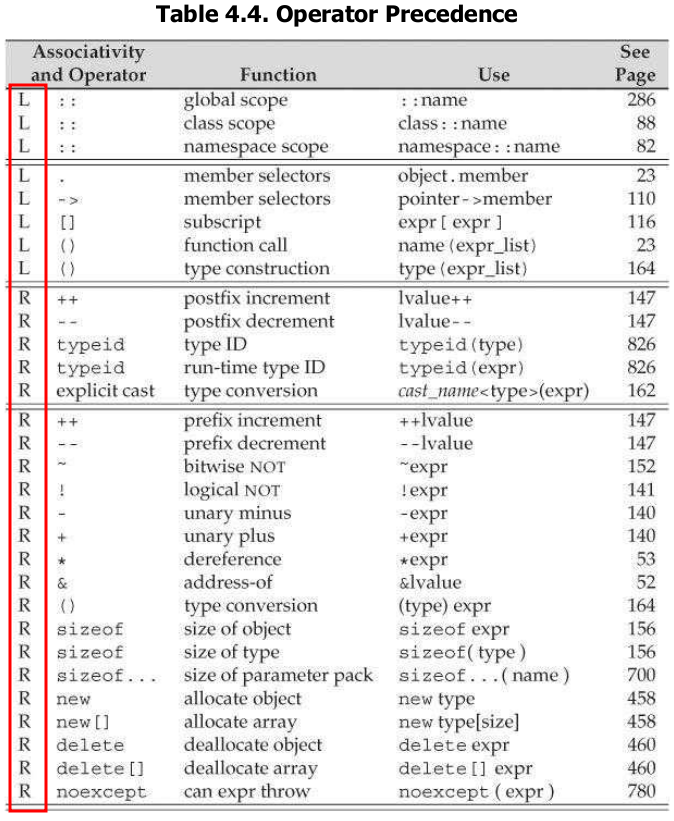
\includegraphics[height=0.7\textheight]{figures/precedence.png}
    \end{figure}
\end{frame}

\begin{frame}{Short-circuit Evaluation}
    Logical operators \texttt{\&\&} and \texttt{||} are short-circuited:
    \begin{itemize}
        \item Both \texttt{\&\&} and \texttt{||} evaluates their left operand first.
        \item If the left operand of \texttt{\&\&} evalutes \blue{\texttt{false}}, the right operand will not be evaluated, and the whole expression evaluates \blue{\texttt{false}}.
        \item If the left operand of \texttt{||} evalutes \blue{\texttt{true}}, the right operand will not be evaluated, and the whole expression evaluates \blue{\texttt{true}}.
    \end{itemize}
\end{frame}

\end{document}